\chapter{Theoretische Grundlagen des Lernens}
\chaptermark{Grundlagen}
Die Erkenntnisse des nachfolgenden Kapitels basieren vor allem 
auf der Psychologie, die einen breiten Forschungsbereich 
in Lerntheorien aufweist. Somit fallen in den nächsten Abschnitten 
oft Verweise auf psychologische Quellen.
Es folgt zuerst eine Erklärung von Begrifflichkeiten des Lernens (Kapitel \ref{BegriffLernen}),
eine Erläuterung zur Entstehung von Lernmotivation und eine kurze 
Einführung ins ARCS-Modell (Kapitel \ref{Lernmotivation}), da RQ2 
die Messung der motivationalen Anreize des 
Lernenden betrifft.
Anschließend folgt eine Begriffsabgrenzung von Lerntypologien (Kapitel \ref{Begriffsabgenzung}) sowie ein 
Überblick zu bekannten Modellen der Lerntypologien (Kapitel \ref{AnalyseLernstilmodelle}) gegeben wird.
Die Betrachtung der verschiedenen Modellen der Lerntypologien ist von Relevanz, um die ausgewählte Lerntypologie des Lernstils sowie  das ausgewählte
ILS-Instrument von Felder und Soloman (1991), welches auf dem Lernstilmodell von Felder und Silverman (1988) beruht, 
zu begründen (Kapitel \ref{AuswahlLernstilmodell}).
Dies ist wichtig, da für 
die Beantwortung von RQ1 ein geeignetes Messinstrument benötigt wird. 
    \section{Definitionen} \label{BegriffLernen}
        \subsection{Lernen} \label{Lernen}
            Lernen ist ein häufig vorkommender Begriff in der Alltagssprache und ein Grundbegriff der Pädagogik.
            Seine Vieldeutigkeit bestärkt sich durch das Vorkommen der hohen Anzahl verschiedenster Ansätze einer Begriffsdefinition.
            Eine eindeutige und präzise allgemeingültige Definition zu finden, ist schwierig. \parencite[103]{Treml.2004} 
            Doch Gemeinsamkeiten in den verschiedenen Definitionen bestehen darin, dass es beim Lernen darum geht, Wissen und Kenntnisse aufzubauen
            und dadurch Verhaltensänderungen durch Erfahrungen entstehen. \parencite[19]{marx.2006}
            In der vorliegenden Arbeit bezieht sich der Begriff Lernen besonders auf den Erwerb von Wissen und Kenntnissen.
            Wissen kann explizit erworben werden, welches 
            sich auf das allgemeine Lernen im Studium, in der Schule oder in einer Fortbildung bezieht und damit relevant für die vorliegende Arbeit ist.
            Treml und Becker (2004) bezeichnen das explizite Lernen \glqq als den bewussten Vorgang der Einprägung von Kenntnissen, der Aneignung und Entwicklung von Wissen, Erkenntnissen, Fertigkeiten, Gewohnheiten und Haltungen.\grqq{} \parencite[106]{Treml.2004} 
            Beim expliziten Lernen hat der Lernende die bewusste Absicht sich neues Wissen anzueignen. Seine volle Aufmerksamkeit ist auf das ihm klar definierte Lernobjekt gerichtet. \parencite[215]{RoehrSendlmeier.2016}
            Die Motivation ist eine notwendige Voraussetzung für jeden Wissenserwerb. \parencite[461]{Reinmann.1998} 
            Die Lernmotivation bekommt somit einen maßgeblichen Stellenwert im Lernprozess. Dahingehend wird seine Bedeutsamkeit in Teilabschnitt \ref{Lernmotivation} näher betrachtet.

        \subsection{E-Learning}
            Das E-Learning findet einen immer höheren Stellenwert in der Lehre und benötigt ein hohes Maß von selbstregulierten Handlungen in der Gestaltung des Lernprozesses. \parencite[34]{marx.2006} 
            E-Learning bezieht sich auf die Art und Weise, wie das Wissen bzw. die Informationen dargestellt, ausgetauscht und vermittelt werden können, und kann als 
            Oberbegriff für alle Varianten und Nutzung digitaler Medien zu Lehr- und Lernzwecken genannt werden. Als digitale Medien werden verschiedene Geräteklassen
            wie Desktop-Computer, Laptop, Tablet oder Smartphone mit entsprechender Periphere wie Beamer oder digitale Tafeln und Technik zur Aufnahme und Wiedergabe 
            von Medien bezeichnet. Sie unterstützen dabei Informationen digital zu speichern, zu verarbeiten und zu präsentieren, sodass an allen existierenden digitalen
            Artefakten gearbeitet werden kann und diese zwischen Menschen ausgetauscht werden können. \parencite[6]{Kerres.2013} 

        
        \subsection{Selbstreguliertes Lernen} \label{selbstgesteurtesLernen}
            Selbstorganisiert, selbstbestimmt, selbstgesteuert, autonom, nicht-organisiert, autodidaktisch, selbst gestalten oder selbst lernen sind teilweise auftretende Synonyme für selbststeuernd.
            Bezogen auf den Lernprozess muss der Lernende Aspekte wie:

            \begin{minipage}[t]{0.5\textwidth}
                \begin{itemize}
                \item das Ziel des Lernprozesses
                \item die Inhalte des Lernprozesses
                \item die Lernzeiten\\
            \end{itemize}
            \end{minipage}
            \hfill
            \begin{minipage}[t]{0.5\textwidth}
                \begin{itemize}
                \item den Lernort 
                \item die Art und Weise des Lernens  
                \end{itemize}
            \end{minipage}
            eigenständig steuern. Somit hängt diese zu steuernde Tätigkeit sowohl von den Anforderungen der jeweiligen Lernumgebung
            als auch von den Merkmalen der Lernenden ab.
            Der Selbststeuerungsgrad hängt davon ab, wieviel der Lernende von den oben genannten Aspekten ohne Fremdeinwirkung selbst zu steuern hat. \parencite[14 f.]{Dietrich.2007} \parencite[195]{Cress.2000}
            Somit fordert das selbstregulierte Lernen vom Individuum, sein Lernen und Denken eigenständig zu regulieren und zu bestimmen. \parencite[45]{Groß.2017} 
            Das selbstregulierte Lernen ist ein allgemeines großes Motivationsproblem (vgl. Kapitel \ref{Problemstellung}).
            Daher soll mithilfe des Prototyps der Arbeit untersucht werden, inwiefern die Motivation des Lernenden bei der Unterstützung der Gestaltung des Lernprozesses beeinflusst werden kann.

        
    \section{Lernmotivation} \label{Lernmotivation}
    Im psychologischen Sinne bezeichnet Heckhausen (1989) Motivation \glqq als eine Sammelbezeichnung für verschiedene Prozesse und Effekte, deren gemeinsamer Kern darin besteht, dass ein Individuum
    sein Verhalten um der erwarteten Folgen willen auswählt und hinsichtlich Richtung und Energieaufwand steuert\grqq{}. \parencite[10]{heckhausen.1989} 
    Im Allgemeinen ist die Motivation die Bereitschaft in einer konkreten Situation eine bestimmte Handlung mit einer bestimmten Intensität durchzuführen. \parencite[4]{tischner.2007} 
    Somit ist die Motivation bestimmend für die Dauer und die Intensität der Lernbereitschaft und den Erfolg beim Lernen. \parencite[44]{Grotian.1999}
    Die vorliegende Arbeit beschäftigt sich mit der Lernmotivation bezüglich des expliziten Lernens und des selbstregulierten Lernens.
    
    \subsection{Modell zur Lernmotivation}
    Das folgende Modell beschreibt einen theoretischen Ansatz, auf welche Art und Weise das selbstregulierte Lernen von Einflussgrößen bestimmt wird und welche Auswirkungen es mit sich zieht.
    
    \begin{figure}[H]   
        \centering
        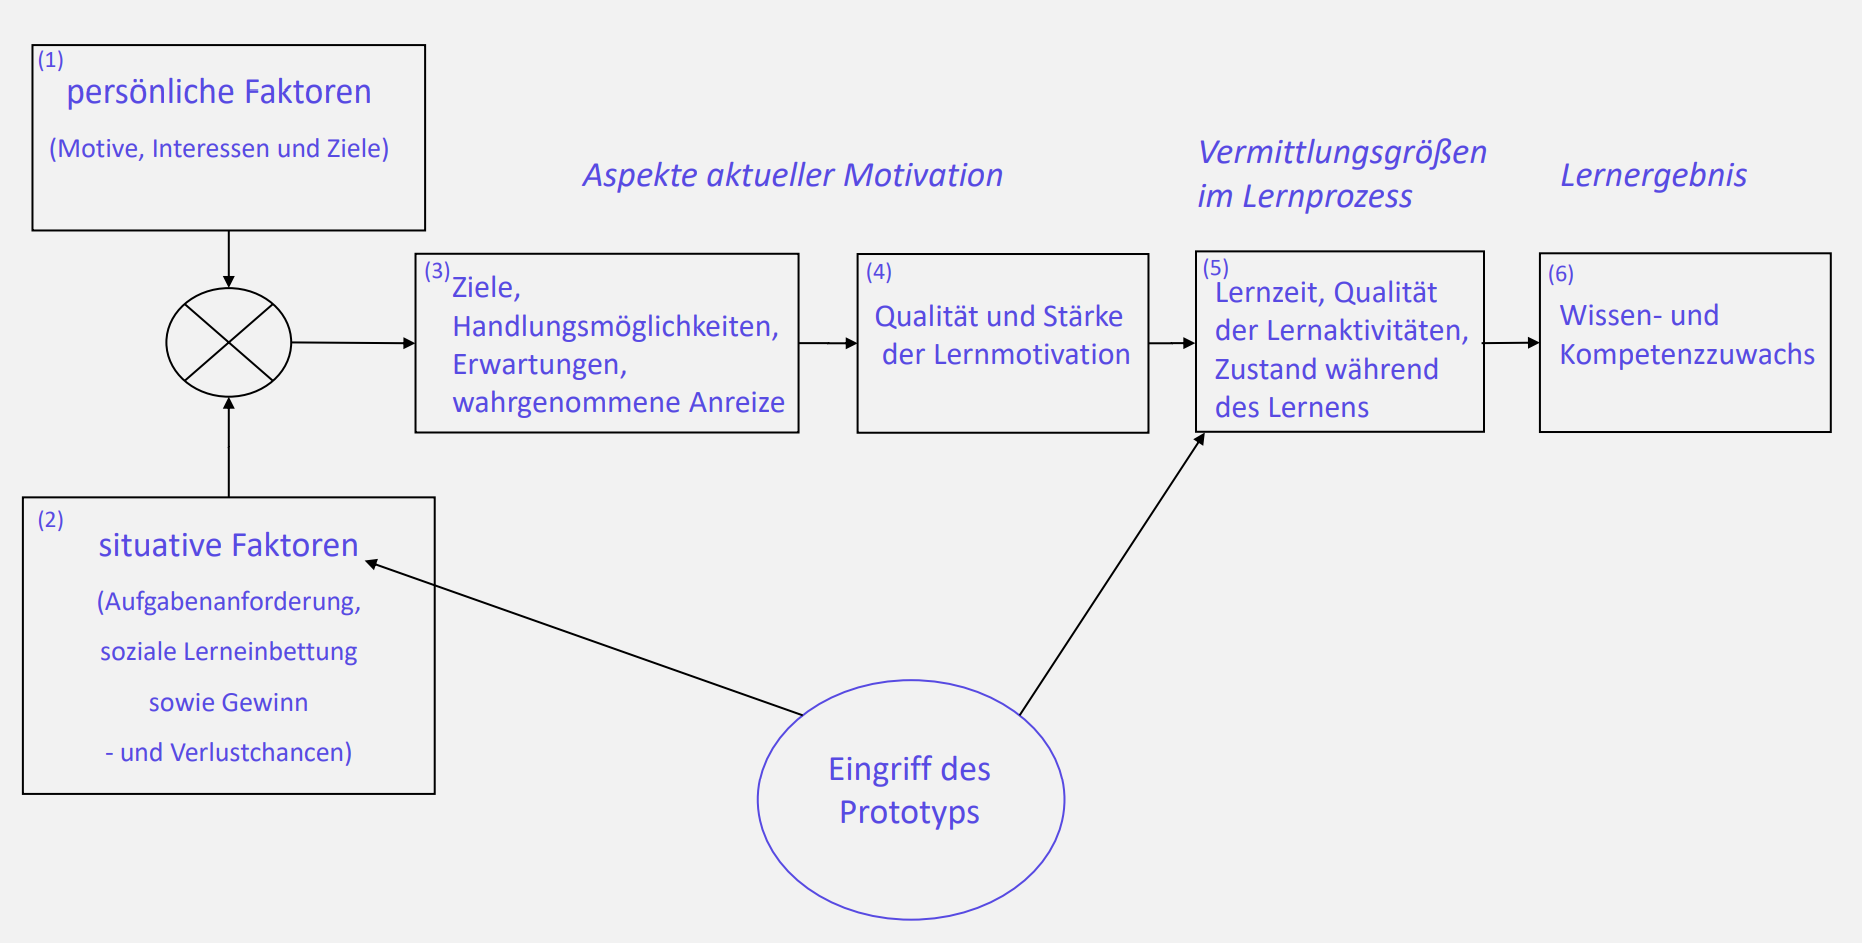
\includegraphics[width=0.6\linewidth]{images/Rahmenmodell_Lernmotivation.png}
        \caption[Modell zur Lernmotivation]{Modell zur Lernmotivation (eigene Darstellung, in Anlehnung an \parencite{rheinberg.2000})}
        \label{fig:Rahmenmodell zu Bedingungen und Auswirkungen von Lernmotivation}
    \end{figure}
    
    In diesem Modell ist erkennbar, dass das motivierte Verhalten sich durch eine Wechselwirkung von persönlichen Faktoren (Box 1) wie Motive, Interessen und Ziele und den situativen Faktoren (Box 2) bedingt.
    Die situativen Faktoren umfassen neben der Struktur und Schwierigkeit der Aufgabenstellung, welche abhängig von den 
    Kompetenzen des Lernenden sind,
    die allgemeine Lernsituation des sozialen Umfeldes (alleine lernen vs. lernen innerhalb einer Gruppe)
    sowie die potentiellen Gewinn- und Verlustchancen, die der Lernende erwarten könnte. Mögliche Gewinnchancen können sein:
    
    \begin{minipage}[t]{0.5\textwidth}
    \begin{itemize}
        \item die eigenen Fähigkeiten kennen zu lernen und sie ggf. zu verbessern
        \item gute Noten zu erreichen\\
    \end{itemize}   
    \end{minipage}
    \hfill
    \begin{minipage}[t]{0.5\textwidth}
        \begin{itemize}
        \item das Lernen über etwas, das man interessant findet
        \item Lob von relevanten Akteuren \\
    \end{itemize}
\end{minipage}

    In welcher Weise sich jeder genannte situative Faktor auf die Lernmotivation des Lernenden auswirkt, hängt von dessen persönlichen Charakterzügen ab. \parencite[83]{rheinberg.2000} 
    Der Prototyp dieser Arbeit greift in den situativen Faktor ein. 
    Er soll als Unterstützung für den Lernenden dienen, 
    indem er die Aspekte des situativen Faktors positiv beeinflusst.
    Zum Beispiel kann der Prototyp den Lernenden dazu
    ermutigen, mehr über seine eigene Art und Weise des Lernens zu erkunden sowie seine Stärken und Schwächen zu 
    identifizieren und dadurch einen höheren Lernerfolg erzielen.
    Darüber hinaus kann der Prototyp 
    als soziale Bezugsperson dienen und ein virtueller Begleiter für den Lernenden werden.
    Je positiver die Einschätzung über die Erwartungen und Anreize, die der Lernende in der Situation wahrnimmt, ausfällt, desto höher ist die Lernmotivation.
    Denn ein gewünschter Kompetenzzuwachs stellt sich ein und die oben genannten Gewinnchancen werden erreicht. 

    Die Interaktion zwischen Personen- und Situationsmerkmalen beeinflussen die Zielsetzung, die Erwartungen des Lernenden und die Anreize, die er in dieser Situation für möglich hält (Box 3). Diese Variablen bestimmen ihrerseits sowohl die Stärke als auch die Qualität der Lernmotivation (Box 4). 
    Also ist die Motivationsstärke dafür entscheidend, wie gut sich Lerntätigkeiten (z.B. 
    das Durcharbeiten eines Textes, vorausgesetzt das Thema ist für den Lernenden interessant), gegenüber konkurrierenden Tätigkeiten (z.B. ein Kinobesuch) durchsetzen können. \parencite[20 f.]{marx.2006} 
        
    Lernmotivation an sich kann keine Lernergebnisse erzeugen. Box fünf stellen Variablen dar, die vermitteln, welchen Einfluss die Lernmotivation auf das Lernen haben kann.
    Im Fall des selbstregulierten Lernens, bei dem der Lernende einen hohen Freiheitsgrad
    in der Art und Weise des Lernens hat, stellen die Zeit und die Art der Lernaktivität eindeutige Variablen dar. \parencite[84]{rheinberg.2000} 
    Der Prototyp der vorliegenden Arbeit kann durch die Bestimmung des individuellen Lernstils des Lernenden 
    eine Tendenz zur richtigen Wahl bezüglich der Art und Weise der Lernaktivität geben. Wird zum Beispiel 
    der Lernstil visuell beim Lernenden identifiziert, kann der Lernende vorerst den Lehrstoff mithilfe
    von visuellen Materialien vertiefen.
    Eine weitere Variable ist der Zustand des Lernenden während des Lernens, der das Lernergebnis beeinflusst.
    Dabei bezieht sich diese Variable auf die physiologische und psychologische Aktivierung und Konzentration des Lernenden während des Lernens. \parencite[84]{rheinberg.2000} 
    Abschließend kann das Lernergebnis den Motivationsprozess weiter fördern, indem der Lernende den erlebten Lernerfolg auf zukünftige Lernsituationen überträgt. Dazu muss der Lernende seinen Lernzuwachs wahrnehmen, indem 
    er die neu gewonnene Leistung mit seinen eigenen vorangegangenen Leistungen vergleicht. \parencite[21]{marx.2006} 

        \subsection{Das ARCS-Modell} \label{Kap2ARCS}
        Aus dem obigen Abschnitt ist deutlich geworden, dass die jeweilige Motivation sowohl zum einen von Merkmalen, Charakteristika und Motiven einer Person abhängt als auch von situativen Faktoren
        beeinflusst wird. 
        Dieses Teilkapitel stellt das ARCS-Modell von Keller (1984) vor, womit die Lernmotivation des Lernenden gemessen werden kann:
        

        \begingroup
        \footnotesize    
        \useunder{\uline}{\ul}{}
        \begin{longtable}{|m{5cm}|m{10cm}|}
        \hline     
        \rowcolor[HTML]{EFEFEF}                                         
        \centering \textbf{Dimension} & \centering \arraybackslash \textbf{ Erläuterung} \\ 
        \hline  \hline 
        Attention (dt. Aufmerksamkeit) & Diese Kategorie bezieht sich auf das Erfassen des Interesses sowie auf die Neugier des Lernenden.
         \\ \hline \hline
        
         Relevance (dt. Relevanz) & Hierbei handelt es sich um die Vermittlung und Bedeutung des Lehrstoffs. Der Lernende soll eine Vorstellung davon bekommen, inwiefern die gezeigten 
         Inhalte mit wichtigen persönlichen Zielen oder Motiven zusammenhängen und somit für ihn eine Relevanz darstellen. 
         \\ \hline \hline

         Confidence (dt. Zuversicht) & Dieser Aspekt meint die Unterstützung der Erfolgszuversicht des Lernenden sowie die Maximierung der Erfolgserwartungen, sodass 
         der Lernende seine gesteckten Ziele aus eigener Anstrengung erreicht. 
         \\ \hline \hline

         Statisfaction (dt. Zufriedenheit) & Die Anstrengung des Lernenden führt zum gewünschten Erfolg und er bleibt motiviert.
         Die Motivation kann dabei aus extrinsischen und intrinsischen Faktoren entstehen. 
         \\ \hline \hline


    \caption[Keller (1984): ARCS-Dimensionen]{Keller (1984): ARCS-Dimensionen (eigene Darstellung, in Anlehnung an \parencite[45 f.]{keller_2010})} 
    \label{tab:/ARCS_Dimensionen_Keller} 
    \end{longtable}
    \endgroup  

       \textbf{Intrinsische und extrinsische Lernmotivation}

        Die Begriffe intrinsische und extrinsische Motivation werden häufig benutzt, allerdings besteht keinerlei Einigkeit darüber, was damit gemeint ist. 
        Möglich ist die folgende Erklärung.
        Aus dem Englischen abgeleitet, bedeuten die beiden Begriffe \glqq innen\grqq{} (engl. intrinsic) und \glqq außen\grqq{} (engl. extrinsic). Die intrinsische Motivation bezieht sich 
        auf Handlungen, die aus der Freude heraus selbst ausgeführt werden. 
        Dazu können sportliche Aktivitäten wie Bergsteigen, Laufen oder auch Aktivitäten wie das Lesen oder Malen gehören, denn der
        Spaßfaktor, welcher während der Tätigkeitsausführung durchlebt wird, ist hoch. 
        Im Gegensatz dazu werden extrinsische Handlungen wegen der erwarteten Folgen ausgeführt. Zum Beispiel kann beim Lernen für eine Klausur das Erreichen einer guten Note, das Abschließen eines Studienmoduls
        oder die Erfüllung der Erwartungen der Eltern den Zweck der Handlungsausübung darstellen. \parencite[5 f.]{Zander2018}

        Das ARCS-Modell dient als Messinstrument, um die Lernmotivation der Probanden in der Studie, welche in Kapitel \ref{Kapitel5.1} aufgeführt wird, zu messen.
        Dies ist von Relevanz, um RQ2 zu beantworten.

    \section{Begriffsabgrenzung von Lerntypologien} \label{Begriffsabgenzung}
    Die Forschung befasst sich mit dem Versuch auf der Basis von verschiedenen theoretischen Modellen mithilfe von Testverfahren, die Art und Weise des Lernens eines Menschen zu klassifizieren, damit dieser dann die Möglichkeit hat, speziell auf seinen Typus
    abgestimmte Lernmethoden zu nutzen und so sein Lernen zu optimieren. Von dieser verlockenden Idee sind viele praktisch tätige Pädagogen überzeugt, die in ihrer täglichen Arbeit interindividuelle Unterschiede bei den Herangehensweisen 
    und Arbeitsweisen der Lernenden beim Lernen feststellen. \parencite[13f.]{Martin.2012}
    Allerdings gibt es keine Einigkeit darüber, welche Verhaltensweisen oder charakteristischen Lernmerkmale in der Klassifikation zur Bestimmung des individuellen Lerntypus miteinbezogen werden sollen. Diese Unstimmigkeit spiegelt sich 
    in der Vielfalt an Ansätzen von theoretischen Modellen  wider und erschwert somit eine eindeutige Abgrenzung der Begrifflichkeiten: Kognitiver Stil, Lernstil, Lernorientierung, Lernpräferenz,
    Lerntyp, Lernstrategie und Lerntaktik. \parencite[9]{Zeiter.2011} \parencite[365]{Cress.2006}
    Creß (2006) unterscheidet einige der eben aufgezählten theoretischen Begrifflichkeiten nach einem Zusammenhang zwischen dem in einer konkreten Situation beobachtbarem Verhalten 
    zu einem situationsübergreifenden Verhalten sowie personenbezogenen Merkmalen. \parencite[365]{Cress.2006} 
    Die nachfolgende Abbildung stellt eine grobe Übersicht der Idee der Unterscheidungsmerkmale dar.
    
    \begin{figure}[H]
        \centering
        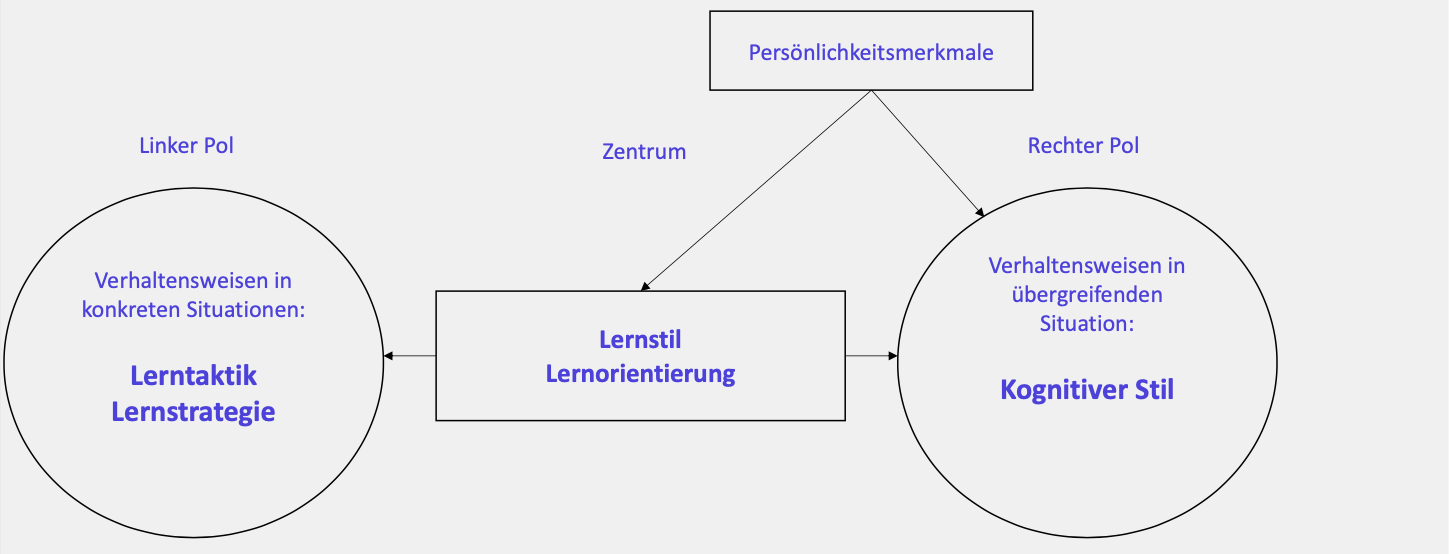
\includegraphics[width=0.8\linewidth]{images/AbgrenzungTheoretischerKonzepte.png}
        \caption[Überblick: Begrifflichkeiten theoretischer Lerntypologien]{Überblick: Begrifflichkeiten theoretischer Lerntypologien (eigene Darstellung, in Anlehnung an \parencite[11]{Zeiter.2011})}
        \label{fig:Überblick Begrifflichkeiten theoretischer Modelle}
    \end{figure}

    Die dargestellte Abbildung zeigt zwei Pole auf, wodurch die Kontradiktion der Verhaltenssituationen verdeutlicht werden soll.
    Der linke Pol steht für die Verhaltensweisen in einer konkreten Situation und der rechte Pol stellt die Verhaltensweisen in übergreifenden Situationen inklusiver Persönlichkeitsmerkmalen dar.
    Die Lerntaktik und Lernstrategie stellen den situationsnahen Pol dar, der Kognitive Stil bildet den anderen Pol. Der Lernstil und die Lernorientierung sind in dem Zentrum der Pole zu finden und 
    zeigen charakteristische Züge. Diese bilden eine Schnittmenge mit den persönlichen Merkmalen, da sie persönliche Charakterzüge aufweisen.
    Im Folgenden werden die einzelnen theoretischen Begrifflichkeiten näher erläutert.

        \textbf{Lernstrategie - und taktik}

            Wild (2006) definiert Lernstrategien allgemein als \glqq jene Verhaltensweisen und Kognitionen, die vom Lernenden aktiv zum Zweck
            des Wissenserwerbs eingesetzt werden.\grqq{} \parencite[427]{Wild.2006} 
            Neben der kognitiven Handlung werden auch Handlungen zur Beeinflussung des motivationalen und affektiven Zustands (z.B. Selbstbelohnung) gezählt. \parencite[5]{Martin.2012} 
            Streblow und Schiefele (2006) fassen folgende gemeinsamen Merkmale in den bestehenden Definitionen der Lernstrategie zusammen:
        
            \begin{enumerate}
                \item Lernstrategien enthalten eine Reihe von effizienten Lerntechniken, welche die Methoden darstellen, die dem Lernenden helfen, die Aufnahme und Verarbeitung des neuen Wissens zu erleichtern. 
                            Beispielsweise ist das Schreiben von Karteikarten (Lerntechnik) für das Auswendiglernen (Lernstrategie) eine oft verbreitete Technik. 
                \item Lernstrategien werden situationsangepasst, zielbewusst und flexibel eingesetzt.
                \item Lernstrategien laufen automatisiert ab. 
                \item Lernstrategien haben das Potenzial bewusstseinsfähig zu werden, sodass die Person die verwendete Lernstrategie soweit verinnerlicht, dass die Handlungen nicht mehr bewusst initiiert und gesteuert werden müssen.
            \end{enumerate} 
            Darüber hinaus werden Lernstrategien in metakognitive und kognitive Strategien sowie in das Ressourcenmanagement unterschieden. \parencite[353]{Streblow.2006} 
            Auf diese wird im späteren Verlauf der Arbeit weiter eingegangen.
            Lernstrategien können gelernt und modifiziert werden und somit der Situation angepasst werden, deshalb beschreiben sie den situationsnahen Pol. \parencite[142]{Looss.2007}
       

        \textbf{Lernstil \& Lernorientierung}

        Der Lernstil einer Person beschreibt weniger die Informationsverarbeitung im Allgemeinen, sondern mehr das individuelle und typische Verhaltensmuster, das eine Person bei Lernaufgaben situationsübergreifend zeigt.
        Diese kognitive und affektive Verhaltensweise der Person stellt ebenfalls charakteristische Züge der Person dar, welche sich als relativ stabil einschätzen lassen. \parencite[142]{Looss.2007}\parencite[58]{Groß.2017}\parencite[365]{Cress.2006} \\
        Als Lernorientierung wird die Art und Weise bezeichnet, in der die Charakterzüge der Person und die Merkmale der Situation ineinander greifen. \parencite[142]{Looss.2007}
        Beide Typologien sind daher dem Zentrum der Abbildung \ref{fig:Überblick Begrifflichkeiten theoretischer Modelle} zuzuordnen.

    
        \textbf{Kognitiver Stil}

        Der Kognitive Stil ist gegenüber der Lernorientierung und dem Lernstil in der Art und Weise der Informationsverarbeitung einer Person allgemeiner gefasst
        und sind daher dem rechten Pol in der Abbildung \ref{fig:Überblick Begrifflichkeiten theoretischer Modelle} zugeordnet. 
        Die allgemeingültige Art des kognitiven Stils zeigt sich als ein gewohnheitsmäßiges und situationsübergreifendes Verhalten und wird als Persönlichkeitsmerkmal gekennzeichnet.\parencite[365]{Cress.2006} 
        Allerdings sind die Konzepte zum Kognitiven Stil nicht empirisch und theoretisch überzeugend. \parencite[339]{tiedemann.2001}
        
        \textbf{Lerntyp \&  Lernpräferenz}

        Einige Autoren verwenden den Begriff Lerntyp auch im Sinne der Lernpräferenz. Aus einer bestimmten Lernpräferenz lassen sich Lerntypen ableiten. \parencite[372]{Cress.2006} 
        Zudem ist eine sehr bekannte verbreitete These, dass sich Lerntypen auf der Basis von Sinneskanälen unterscheiden lassen.
        Allerdings fehlt es an logischer und empirischer Evidenz diese These zu beweisen.
        Dennoch genießt diese Lerntypentheorie, welche auf den Autor Vester (1998) zurückzuführen ist, ein hohes Maß an Popularität. \parencite[144]{Looss.2007} \nocite{Vester.1998}
        Vester (1998) behauptet eine Abhängigkeit des individuellen Lernerfolgs und der persönlichen Lernpräferenz von unterschiedlichen Wahrnehmungskanälen zu erkennen. Daraufhin definiert er vier 
        unterschiedliche Lerngruppen und unterscheidet zwischen dem visuellen, optischen, haptischen und intellektuellen Lerntyp. \parencite[144]{Looss.2007} \parencite[17]{Schrader.2008} \parencite[372]{Cress.2006} 
        Der Begriff der Lernpräferenz wird beispielsweise oft in Verbindung mit den Ansätzen von Vester (1998) und Neber (1994) gebracht. Bei Neber (1994) wird nach der Präferenz für autonomes Lernen 
        oder Lernen in der Gruppe unterschieden. \nocite{Neber.1994}
        Allerdings sind die Versuche, Lerntypen über Lernpräferenzen zu ermitteln theoretisch wenig fundiert. \parencite[375]{Cress.2006}  
            
        Zusammenfassend ist an dieser Stelle zu erwähnen, dass die Lerntypologien: Kognitiver Stil, Lerntyp und Lernpräferenz aufgrund von zu wenig fundierter Überzeugungskraft nicht 
        als weitere mögliche Typologie in Frage kommen und deshalb nicht für die Begründung der ausgewählten Lerntypologie beachtet werden.
        
        \section{Analyse historischer bekannter Modelle der Lerntypologie} \label{AnalyseLernstilmodelle}

    Die  Forschungsansätze der Lernstrategie und -stiltheorien nehmen ihren Verlauf bis zur Antike. 
    So folgt eine Einschränkung auf die theoretischen Konzeptionen der letzten 50 Jahre in der Geschichte. Es herrschen zwei dominierende Forschungsstränge: 
    \textbf{\glqq Approach to Learning-Ansätze\grqq{}} und \textbf{\glqq Kognitionspsychologische-Ansätze\grqq{}}.
    Der  \textbf{ Approach to Learning (ATL)} Ansatz beschreibt das unterschiedliche Lernverhalten der Menschen. Dieses unterschiedliche 
    Lernverhalten kann in verschiedenen Situationen beobachtet werden und weist einen
    Bezug zu den jeweiligen Persönlichkeitszügen des Lernenden auf. 
    Die Identifikation mit seinen charakteristischen Merkmalen steht im Vordergrund. 
    Die  \textbf{kognitiven Ansätze} beziehen sich hauptsächlich auf die Frage, wie der Lernprozess allgemein funktioniert und optimiert werden kann. Dabei wird die Vorgehensweise von Informationsaufnahme über die
    Verarbeitung bis hin zur Speicherung sowie den Möglichkeiten zur Beeinflussung dieses Prozesses untersucht. In vielen nachfolgenden Konzepten wird keine klare Trennung bezüglich der Methoden und Ziele der beiden 
    Forschungsrichtungen geschaffen. \parencite[8]{Martin.2012} 
    Die nachfolgende Abbildung zeigt wichtige Vertreter der Lernstrategie und -stilforschung in chronologischer Abfolge. Anschließend werden die Grundgedanken der Befunde kurz erläutert, um 
    die geeignete Lerntypologie und das geeignete Modell zu begründen, welche für die Beantwortung von RQ1 relevant sind. 

    
    \begin{figure}[H]
        \centering
        \includegraphics[width=0.8\linewidth]{images/timeline.png}
        \caption[Timeline: Vertreter von Lerntypologie-Modellen]{Timeline: Vertreter von Lerntypologie-Modellen (eigene Darstellung)}
        \label{fig:Timeline: Vertreter von Lerntypologie-Modellen}
    \end{figure}

        \subsection{Approach to Learning Ansätze} \label{ATL}
        \textbf{Marton \& Säljö (1976)} entdeckten zwei grundlegende Herangehensweisen an das Lernen: \textbf{\glqq Surface-Approach\grqq{} } (dt .Oberflächenverarbeitung) und 
        \textbf{\glqq Deep-Approach\grqq{} } (dt. Tiefenverarbeitung). \nocite{Marton.1984}
        Die erste Kategorie beschreibt eine auf Wiederholung und Auswendiglernen ausgerichtete Herangehensweise, die  weniger am tiefen Verstehen und mehr an der exakten Wiedergabe von losen Fakten interessiert ist.
        Die zweite Kategorie zeigt ein Verhaltensmuster, wodurch der Lernende Zusammenhänge und Querverbindungen zu seinem Vorwissen versucht zu verknüpfen. Er ist an dem Verstehen der Informationen interessiert. \parencite[8 f.]{Martin.2012}\parencite[366]{Cress.2006}\parencite[145 f.]{Looss.2007}
        
        Unabhängig von Marton \& Säljö (1976), jedoch zu derselben Zeit, identifiziert der Brite \textbf{Pask (1976)} zwei Lernstrategien \textbf{\glqq holistic\grqq{}} (dt. ganzheitlich) und \textbf{\glqq serialistic\grqq{}} (dt. serialistisch). Dabei bezeichnet er Personen, welche die holistic Strategie wiederholt anwenden als \textbf{\glqq Comprehension Learner\grqq{}}. 
        Dieses Lernverhalten zeichnet sich durch eine globale Lerneinstellung aus. Das Lernen ist reich an Ankedoten, Illustrationen und Analogien.
        Anwender der serialistic Strategie werden als \textbf{\glqq Operating Learner\grqq{}} beschrieben. Dieses Lernverhalten ist durch die sukzessive Bearbeitung des Lernstoffes geprägt. Der Lerner arbeitet kleinschrittig und 
        beginnt beim Detail, bevor er zum Gesamten übergeht. Pask
        (1976) ist ein Befürworter eines flexiblen Lernverhaltens und bezeichnet Personen, die
        je nach Aufgabenstellung entweder die holistic oder serialistic Strategie anwenden als
        \textbf{\glqq Versatile Learner\grqq{}}.
        Die beiden Lernstile Comprehension Learner und Operating Learner sind mit den Dimensionen von Surface- und Deep-Aproach vergleichbar.
        \parencite[9]{Martin.2012}\parencite[369]{Cress.2006}\parencite[12 f.]{Thielke.2003} 

        Gestützt auf die Untersuchungen von Marton \& Säljö (1976) und Pask (1976), die als Orientierungsansätze für die weitere Forschung gelten, unternahm die britische Forschungsgruppe um \textbf{Entwistle \& Ramsden (1983)} den Versuch anhand von faktoranalytischen Methoden\footnote{Faktoranalysen gehören zu den Methoden der multivarianten Statistik und dienen dazu, aus einer empirischen Beobachtung von vielen verschiedenen manifesten Variablen auf wenige zugrunde liegende latente Variablen zu schließen. Vgl. \url{https://eric-klopp.de/texte/explorative-faktorenanalyse.php}, aufgerufen am 04.11.2021},
        einen quantitativen Fragebogen zur 
        Erfassung der Herangehensweisen an das Lernen im Sinne der obigen ATL-Dimensionen zu erstellen. Der \textbf{\glqq Approaches to Studying\grqq{}  (ASI)}  Fragebogen von Entwistle \& Ramsden (1983) sollte die Erhebung 
        des Lernverhaltens von größeren studentischen Stichproben ermöglichen. Die Auswertung der Pilotstudie ergab eine systematische Verknüpfung von Lernmotivation und Lernverhalten. \parencite[9]{Martin.2012}\parencite[368 f.]{Cress.2006} 

        Gleichzeitig entwickelte die australische Forschergruppe um \textbf{Biggs (1987)} einen ähnlichen Ansatz zu den oben genannten Lernorientierungen. \nocite{Biggs.1987}
        Er forderte die Verknüpfung von Lernmotivation und spezifischem Lernverhalten zu einer distinkten Herangehensweise an eine Lernaufgabe und stellte dabei drei Dimensionen fest. Er unterschied zwischen 
        dem \textbf{\glqq Surface-Approach\grqq{}}, dem \textbf{\glqq Deep-Approach\grqq{}} und dem \textbf{\glqq Achieving-Approach\grqq{}} (dt. Erfolgreicher-Ansatz).
        Diese Ansätze hat er in seinem  \textbf{\glqq Study Process Questionnaire\grqq{} (SPQ)} mit je einer motivationalen und einer strategischen Skala abgebildet. \parencite[10]{Martin.2012}\parencite[367 ff.]{Cress.2006} 
        Der Surface- und Deep-Approach beziehen sich auf die Art der Auseinandersetzung mit dem Lernstoff und entsprechen somit den Konzepten von Marton \& Säljö (1976). \parencite[383]{Wild.2000}
        Der Achieving-Approach wirkt sich nicht sehr stark auf den Lernprozess aus, sondern dient der Strukturierung der räumlichen und zeitlichen Rahmenbedingungen und ähnelt somit dem Konzept des Versatilen Lerners von Pask (1976). \parencite[15]{Thielke.2003}
        
        Aufgrund einer hohen Anzahl an Studienabbrüchen in der schwierigen Ingenieurausbildung in den USA entwickelten 
        \textbf{Felder und Silverman (1988) (FS)} ein theoretisches Lernstilmodell speziell für diese Ausbildung. Das FS-Modell klassifiziert 
        auf einer Skala, in welcher Form Lernende Informationen aufnehmen. \parencite[21 f.]{Felder.1995} \parencite[674]{Felder.1988}
        \textbf{Felder und Soloman (1991)} entwickelten ein Instrument namens \textbf{\glqq Index of Learning Styles\grqq{} (ILS)} zur Bewertung dieses 
        Lernstilmodells. \parencite[2]{Felder.2002}
        Folgende vier
        Lernstile\footnote{Die Dimensionen induktiv/deduktiv wurden entfernt und die Dimensionen visuell/auditiv wurde in visuell/verbal geändert. \parencite[1 f.]{Felder.2002}} werden definiert: 
        
        \begingroup
            \footnotesize    
            \useunder{\uline}{\ul}{}
            \begin{longtable}{|m{3cm}|m{12cm}|}
            \hline     
            \rowcolor[HTML]{EFEFEF}                                         
            \centering \textbf{Dimension} & \centering \arraybackslash \textbf{ Erläuterung} \\ 
            \hline  \hline 
            Sensorisch/ intuitiv &  \textbf{Sensorische Lerner} bedienen sich detailreicher Fakten, Daten und Informationen. Sie haben eine sorgfältige und fleißige Arbeitsstruktur sowie sie die Lernstrategie des Auswendiglernens nutzen. Um wissenschaftliche Methoden korrekt anzuwenden, fordern sie in diese eine gute Einführung und lehnen Aufgabengebiete, die in Lehreinheiten nicht behandelt wurden, ab. \textbf{Intuitive Lerner} zeigen ein gegensätzliches Verhalten zum sensorischen Lerner auf. Sie versuchen 
            Auswendiglernen und Wiederholungen zu umgehen. Des Weiteren bevorzugen sie Theorien und Konzepte, um eigenständig
            Schlüsse aus den Informationen zu ziehen sowie von komplexeren Aufgaben herausgefordert zur werden. 
             \\ \hline \hline
            Visuell/ verbal & \textbf{Visuelle Lerner} bevorzugen die Präsentation von Informationen in Bildern, Diagrammen, Flussdiagrammen, Zeitleisten, Filmen und Demonstrationen. \textbf{Verbale Lerner} ziehen schriftliche oder gesprochene Erklärungen vor. 
            \\ \hline \hline
            Aktiv/ reflektiv &  \textbf{Aktive Lerner} bevorzugen in Lernsituationen, die ihnen ermöglichen, etwas Aktives zu tun, zum Beispiel eine Teilnahme an einer Diskussion über das Thema oder jemandem etwas zu erklären.
            Sie bevorzugen Gruppenarbeit. \textbf{Reflektive Lerner} benötigen eine Gelegenheit, in der sie vorerst über die Informationen nachdenken können. Sie bevorzugen es alleine zu arbeiten.
            \\ \hline \hline
            Sequentiell/ global & \textbf{Sequentielle Lerner} lösen Probleme Schritt für Schritt, damit sie den klaren linearen Zusammenhang erkennen können. Durch diesen logischen Aufbau können sie mehr Informationen aufnehmen. \textbf{Globale Lerner} können Probleme schnell anhand des Gesamtbildes lösen. Allerdings haben sie Probleme, Einzelheiten ihres Denkprozesses zu erläutern.
            \\ \hline \hline
        \caption[Felder und Silverman (1988): FS-Dimensionen]{Felder und Silverman (1988): FS-Dimensionen (eigene Darstellung, in Anlehnung an \parencite[22 ff.]{Felder.1995})} 
        \label{tab:/ILS-Dimensionen} 
        \end{longtable}
        \endgroup  
        
        Im Folgenden wird der zweite Forschungsstrang vorgestellt, um die ausgewählte Lerntypologie zu begründen.

        \subsection{Kognitionspsychologische Ansätze }
        In den 1980er Jahren
        entwickelten \textbf{Weinstein und Mayer (1986)} in den USA  einen neuen Forschungsstrang, der das Lernen explizit als Informationsverarbeitungsprozess verstand.
        Die Beeinflussung des  Enkodierungsprozesses\footnote{Der Enkodierungsprozess ist die Übersetzung der neuen Sinneseindrücke in neuronalen Code, sodass das Gehirn die neuen Informationen verarbeiten kann. \parencite[178]{berting.2011}}
        beim Erwerb neuer Informationen war die Grundlage dieses Ansatzes. Der Prozess kann in \textbf{Selektion}, \textbf{Erwerb}, \textbf{Konstruktion} und   \textbf{Integration}  eingeteilt werden.
        Bei der\textbf{ Selektion} achtet der Lernende aktiv auf neue Informationen, die auf die Sinnesrezeptoren\footnote{ Sinnesrezeptoren dienen der Wahrnehmung von Umweltereignissen. \parencite[90]{Roth.1997}}
                einwirken und überträgt diese Informationen ins Arbeitsgedächtnis\footnote{Das Arbeitsgedächtnis dient dem Halten und Austauschen von Informationen für kurzzeitige Tätigkeiten und Entscheidungen. \parencite[290]{Kircher.2007}}
        Bei dem \textbf{Erwerb} überträgt der Lernende die Informationen aktiv vom Arbeitsgedächtnis ins Langzeitgedächtnis für dauerhafte Speicherung.
        Bei der \textbf{Konstruktion} baut der Lernende  aktiv Verbindungen zwischen den Ideen in den Informationen, die das Arbeitsgedächnis erreicht haben, auf (Sinneinheiten).
        Bei der \textbf{Integration} sucht der Lernende aktiv nach Vorwissen in seinem Langzeitgedächnis, um diese in das Arbeitsgedächnis zu laden und die neuen Sinneinheiten mit bestehendem Wissen zu verknüpfen.  \parencite[317]{Weinstein.1986} \parencite[17]{Thielke.2003}
        
        Verschiedene Lernstrategien\footnote{ Können als Verhaltensweisen und Kognitionen definiert werden, auf die sich ein Lernender während des Lernens einlässt, um den Kodierungsprozess des Lernenden zu beeinflussen. \parencite[315]{Weinstein.1986}}
        können die aufgezählten Phasen unterstützen. Dadurch ist es möglich ein persönliches Lernverhalten zu erzeugen. Dieses persönliche 
        Lernverhalten kann gemessen werden. 
        Ein geeignetes Messinstrument ist für die Beantwortung von RQ1 notwendig. Für die Begründung des ausgewählten Messinstruments bedarf es einer weiteren Analyse der kognitionspsychologische Ansätze.
        Die kognitiven Strategien lassen sich in \textbf{Wiederholungs-}, \textbf{Elaborations-} und \textbf{Organisationsstrategien} unterscheiden.
        Wiederholungsstrategien können gezielt zur Selektion und zum Erwerb von Informationen eingesetzt werden,
        während Elaborations- und Organisationsstrategien sich für die Konstruktions- und Integrationsphase eignen. 
        \textbf{Unterstützungsstrategien}, die benötigt werden, um die Aufmerksamkeit möglichst lange aufrecht zu halten
        und somit eine günstige Motivationslage für das Lernen zu schaffen, können auf alle vier Phasen angewendet werden. \parencite[317]{Weinstein.1986} \parencite[17]{Thielke.2003}

        \textbf{Weinstein, Palmer und Schulte (1987)} entwickelten das \textbf{\glqq Learning and Study Strategies Inventory\grqq{} (LASSI)}
        zur quantitativen Erfassung der aufgeführten Strategien. \parencite{WeinsteinPalmerSchulte.1987}
        Trotz methodischer Schwächen bildet die Taxonomie hinter LASSI die Grundlage für die heute verwendeten kognitionspsychologischen
        Lernstrategiekategorisierungen. \parencite[11]{Martin.2012}

        Die Forschungsgruppe um \textbf{Pintrich (1991)} verfeinerte die Ansätze von Weinstein und Mayer (1986) und untermauerte diese empirisch in Form des \textbf{\glqq Motivated Strategies for Learning Questionnaire\grqq{} (MSLQ)}, welches ein statistisches und qualitatives Instrument darstellt. Pintrich u.a. (1991) unterschieden die Lernstrategien zwischen \textbf{kognitiver}, \textbf{metakognitiver}, \textbf{ressourcenorientierter} und 
        \textbf{motivationaler} Kategorie. 
        Dabei blieben die kognitiven Strategien unverändert.
        Die metakognitiven Lernstrategien dienen der Planung, Überwachung und Regulation. 
        Die ressourcenorientierten Lernstrategien wurden in interne und externe Komponenten unterteilt und haben das Ziel, das Lernen von störenden Einflüssen abzuschirmen oder durch die Herbeiführung von externer Hilfe zu unterstützen. \parencite[12]{Martin.2012}\parencite[370]{Cress.2006} \nocite{Pintrich.1991}
        
        \textbf{Wild und Schiefele (1994)} entwickelten auf Basis des MSLQ das deutschsprachige Erhebungsinstrument \textbf{\glqq Lernen im Studium\grqq{} (LIST)}, welches nur die kognitiven und nicht die 
        motivationalen Skalen des MSLQ enthält. 
        Mithilfe dieses Instruments war es möglich, eine größere Anzahl von Personen zu testen. \parencite[12]{Martin.2012}\parencite[370]{Cress.2006} \nocite{Pintrich.1991}

        \textbf{Creß und Friedrich (2000)} wählten ebenfalls diese Methode und führten eine Untersuchung an ca. 2000 Fernstudierenden durch. Für die Klassifikation der Gruppen setzten sie 
        kognitive, metakognitive und ressourcenorientierte Skalen des LIST ein, nahmen eine MSLQ-basierte Skala zur Messung der intrinsischen Lernmotivation sowie eine eigene Skala
        zur subjektiven Lernkompetenz. \parencite[370]{Cress.2006} Mithilfe einer  \textbf{Clusteranalyse} definierten sie folgende Gruppen: 
        
        \begingroup
        \footnotesize    
        \useunder{\uline}{\ul}{}
        \begin{longtable}{|m{2cm}|m{13cm}|}
        \hline     
        \rowcolor[HTML]{EFEFEF}                                         
        \centering \textbf{Gruppen} & \centering \arraybackslash \textbf{ Erläuterung} \\ 
        \hline  \hline 
        Minimax-Lerner & Diese Gruppe verwendet wenig kognitive und metakognitive Strategien, strengen sich durchschnittlich an, haben eine hohe subjektive Lernkompetenz und erzielen 
        mit wenig Lernzeit eine überdurchschnittliche Lernleistung.
         \\ \hline \hline
         Tiefen-verarbeiter & Diese Gruppe wendet alle Strategien bis auf die Wiederholungsstrategie häufig an. Sie haben eine hohe subjektive Lernkompetenz, sind intrinsisch motiviert und haben eine hohe Lernzeit und -leistung. Diese Gruppe umfasst den Großteil der Studierenden. Auch so haben sie die größte Gemeinsamkeit mit dem \glqq Deep-Approach\grqq{} des ATL-Ansatzes.

        \\ \hline \hline
        Wiederholer &  Diese Gruppe verbringt viel Zeit mit Wiederholen anstatt mit Elaborieren. Sie ist extrinsisch motiviert, verwendet viel Lernzeit mit unterdurchschnittlichem Erfolg und strahlt eine subjektive Unsicherheit aus. Die \glqq Surface-Approach\grqq{} -Gruppe der ATL-Ansätze ähnelt dieser Gruppe.

        \\ \hline \hline
        Minimal-Lerner & Diese Gruppe verwendet wenige Lernstrategien und hat eine geringe subjektive Lernkompetenz. Sie weisen eine geringe Lernzeit mit niedrigem Erfolg auf.

        \\ \hline \hline
    \caption[Cress und Friedrich (2000): Clusteranalyse]{Cress und Friedrich (2000): Clusteranalyse (eigene Darstellung, in Anlehnung an \parencite[370]{Cress.2006})} 
    \label{tab:/Cluster-Dimensionen} 
    \end{longtable}
    \endgroup  

    Mit dieser Taxonomie kamen Cress und Friedrich (2000) auf ähnliche Ergebnisse wie Pintrich u.a. (1993) und konnten so den Deep- und Surface-Approach der ATL-Forscher erneut aufzeigen. Jedoch kritisiert Cress (2006) diese starken Zusammenhänge zwischen den Konzepten, da die Analysen auf Selbstberichten der Lernenden über ihren Strategieeinsatz beruhen. Dies hat zur Folge, dass die Validität der durch Selbstberichte erfassten 
    Lerntypen schwindet. \parencite[370 f.]{Cress.2006} \parencite[15 f.]{Martin.2012} Allerdings stimmt die Methode der Selbstberichte und das tatsächliche Vorgehen nicht immer 
    überein. Zudem kann das Wissen über die Lernstrategien oftmals unvollständig sein oder der konkrete Einsatz der Strategie wird gar nicht vorgenommen. \parencite[148]{Looss.2007}\nocite{Pintrich.1993}

    \section{Auswahl einer Lerntypologie \& eines Modells} \label{AuswahlLernstilmodell}
 
    Die beiden Lernorientierungen Deep- und Surface-Approach konnten empirisch gestützt werden. Allerdings 
    wurden bei der Entwicklung des ASI-Fragebogens von Entwistle \& Ramsden (1983) sowie des SPQ-Fragebogens von Biggs (1987) auf der Seite der ATL-Ansätze,
    verschiedene Erkenntnisse aus der differentiellen Psychologie, der Motivationspsychologie und der Lernverhaltensforschung verwendet.
    Dies führt zu schwammigen und zu wenig stringenten Konstrukten. Zudem wurden theoretisch hergeleitete Skalen mit 
    faktoranalytisch gewonnenen Skalen kombiniert. Dies führt zu einer generellen Unschärfe, wodurch es schwierig ist, kausale Zusammenhänge zwischen Lernverhalten und Lernmotivation
    zu untersuchen. Abschließend stellten sich ASI als auch SPQ als wenig reliable Erhebungsinstrumente heraus. \parencite[10]{Martin.2012} Daher wird die Typologie der Lernorientierung im Folgenden 
    nicht weiter betrachtet.
    
    Die kognitionspsychologischen Ansätze haben zu einer stärkeren theoretischen Fundierung der Lernstrategie-Forschung geführt. \parencite[13]{Martin.2012}
    Daher ist eine Kombination des Fragebogens LIST von Wild und Schiefele (1994) und MSLQ von Pintrich (1991) mit anschließender Einteilung der identifizierten Lernstrategien in die Lernstilklassifikation
    nach Cress und Friedrich (2000) möglich. Allerdings ist diese genannte Möglichkeit sehr aufwendig bezüglich der Durchführung, 
    da der LIST-Fragebogen über ca. 80 Fragen enthält. Selbst 
    Friedrich und Creß (2000) konnten damals keine Originalskalen dieses Ansatzes verwenden. Stattdessen wurden aus bestehenden Instrumenten Kurzskalen aus denjenigen Items gebildet, die für die Analyse der Fernstudierenden relevant waren, und 
    auf die Originalskalen von LIST die höchste Beeinflussung hatten.
    Aufgrund des großen Umfangs und des zusätzlichen Aufwands für eine mögliche Adaption des LIST-Fragebogens, welcher nicht Bestandteil der Zielsetzung der vorliegenden Arbeit ist, 
    wird dieser Ansatz nicht für das weitere Vorgehen dieser Arbeit verfolgt. Somit entfällt die Typologie der Lernstrategien und -taktiken.
    Hingegen wird das FS-Modell von Felder und Silverman (1988), welches einen ATL-Ansatz darstellt, häufig bei technologiegestützten Lernsystemen verwendet. \parencite[866]{Funda.2009}
    Beispiele sind: 
    \begin{itemize}
        \item CS383 von Carver u.a. (1996) stellt einen E-Learning-Kurs vor, welcher auf dem persönlichen Lernstil des Lernenden basiert. \nocite{Carver.1996}
        \item CooTutor von Wang u.a. (2006) lehrt räumliche geometrische Transformationen in einer webbasierten Lernumgebung. Die Lernstrategie passt sich dabei an den Lernstil des Lernenden an. \nocite{Wang.2006}
        \item Li u.a. (2010) berichten über einen E-Learning-Kurs zur Anpassung an den Lernstil des Lernenden. \nocite{Li.2010}
        \item Oscar von Latham u.a. (2010) bestimmt in einem Nachhilfegespräch den Lernstil eines Lernenden dynamisch und passt sich im weiteren Verlauf an den identifizierten Lernstil an. %\parencite{Oscar}
    \end{itemize} 

    Die Popularität der Verwendung des FS-Modells begründet sich darin, dass sich
    die Dimensionen vom FS-Modell voneinander unterscheiden lassen und somit eine starke Unabhängigkeit voneinander zeigen.
    Des Weiteren enthält jede FS-Dimension eine genaue Beschreibung zu seinem typischen Verhalten, was
    bei der Klassifikation des Lernstils eines Lernenden unterstützend wirkt. 
    Außerdem ist es einfacher, eine kleine Anzahl von Dimensionen zu implementieren, die das FS-Modell aufweist. \parencite[14]{Latham.2011}
    Das FS-Modell basiert auf der Typologie des Lernstils, daher wird die Typologie der Lernorientierung nicht weiter beachtet.
    Schlussfolgernd wird für das weitere Vorgehen und für die Implementierung des Prototyps das FS-Modell, das ILS-Instrument sowie der Begriff des Lernstils verwendet.

    \textbf{Kapitelzusammenfassung} 
    \begin{itemize}
        \item Lernen bezieht sich besonders auf den Erwerb von Wissen und Kenntnissen. Wissen kann explizit erworben werden, welches sich auf das allgemeine Lernen im Studium, in der Schule oder in einer Fortbildung bezieht.
        \item E-Learning hat einen hohen Stellenwert in der Lehre und stellt einen Oberbegriff für alle Varianten und Nutzungen digitaler Medien zu Lehr- und Lernzwecken dar. Ein hoher Grad an den Kompetenzen des selbstgesteuerten Lernens spielen eine bedeutende Rolle im E-Learning-Format.
        \item Selbstgesteuertes Lernen fordert vom Lernenden, sein Lernen und Denken eigenständig zu regulieren und zu bestimmen. Dabei muss der Lernende Aspekte wie: 
        das Ziel des Lernprozesses, die Inhalte des Lernprozesses, die Lernzeiten, den Lernort sowie die Art und Weise des Lernens selbstständig steuern. Der Prototyp der vorliegenden Arbeit kann in den eben genannten Aspekten unterstützend wirken.
        \item Nach Rheinberg, Vollmeyer und Burns (2000) ist das motivierte Verhalten durch die persönlichen Faktoren und die situativen Faktoren bestimmt. Der Prototyp kann zum einen den situativen 
        Faktor beeinflussen und zum anderen eine Tendenz zur richtigen Wahl bezüglich der Art und Weise der Lernaktivität geben.
        \item Das ARCS-Modell besteht aus den Dimensionen: Attention, Relevance, Confidence und Statisfaction.
         Die Entstehung von Lernmotivation sowie das ARCS-Modell zur Messung der Lernmotivation wurden beschrieben, um die Generieung und Auswahl der Items für die, im Kapitel \ref{Kapitel5.1} aufgeführte Umfrage, nachvollziehen zu können. Des Weiteren werden Messinstrumente für die Beantwortung für RQ2 benötigt.
        \item Modelle der Lerntypologie unterteilen sich in \glqq Approach to Learning-\grqq{} und in \glqq Kogni-tionspsychologische-Ansätze\grqq{}.
        \item Die Betrachtung der verschiedenen Modellen der Lerntypologien war von Relevanz, um den Lernstil sowie das 
        FS-Modell, welches im Prototypen implementiert wird, zu begründen.
        Dies ist wichtig, da für die Beantwortung von RQ1 ein geeignetes Modell benötigt wird.

    \end{itemize}

    



